\documentclass{report}   %Documento tipo reporte
\usepackage[spanish]{babel}    %Paquete de Idioma
\usepackage{float, graphicx, caption, color, amsmath}
\usepackage[hidelinks]{hyperref}

\begin{document}


\begin{titlepage}    %Portada
	\centering
	{\huge\bfseries PROYECTO DE INVESTIGACIÓN: \par}
	\vspace{1cm}
	{\huge\bfseries HILOS \par}
    \vspace{3cm}
    {\scshape\large Valentina Botero Vivas \par}
    \vspace{3cm}
      {\scshape\large Docente  \par}
	\vspace{0.5cm}
    {\scshape\large Augusto Salazar Jimenez  \par}
	\vspace{3cm}
	 {\scshape\large Universidad de Antioquia \par}
	\vspace{1cm}
    {\scshape\large Informática II  \par}
	\vspace{1cm}
	{\scshape\large 16 de Julio del 2020 \par}
\end{titlepage}
Los hilos o subprocesos son  el flujo de control de datos de un programa. Es un medio que permite administrar las tareas de un procesador y de sus diferentes núcleos de una forma más eficiente.\\ Gracias a los hilos, las unidades mínimas de asignación, que son las tareas o procesos de un programa, pueden dividirse en trozos para así optimizar los tiempos de espera de cada instrucción en la cola del proceso.\\

Ahora cada hilo contiene un trozo de la tarea a realizar, algo más simple de realizar que si introducimos la tarea completa en el núcleo físico. De esta forma el sistema es capaz de procesar varias tareas al mismo tiempo y de forma simultánea, de hecho, podrá hacer tantas tareas como hilos tenga, y normalmente son una o dos por cada núcleo.\\
Aunque un núcleo solo puede realizar una tarea a la vez, se pueden usar los hilos para hacer creer al usuario (y al ordenador) que sí se puede hacer más de una tarea al mismo tiempo.\\
En lugar de realizar una tarea al completo, se divide en porciones ( cada hilo se encarga de un aspecto concreto del programa ), de modo que se van alternando entre porciones de distintas tareas para que parezca que ambas se están ejecutando simultáneamente.


Tienen una desvantaja y es que están limitados por las capacidades del sistema donde se corren.

\section*{Historia}
En un sistema multiprogramado, los procesos constituyen una forma de expresar concurrencia, es decir,la capacidad de diferentes partes para ejecutarse fuera de orden o en orden parcial, sin afectar el resultado final. Sin embargo, hace más de medio siglo, el concepto de proceso no fue desarrollado para permitir la convivencia de los programas de distintos usuarios sobre los carísimos computadores de la época. Estos programas también se ejecutaban en concurrencia, pero solo interaccionaban entre ellos en su competencia por el acceso a los recursos compartidos. Sin embargo, enseguida se vio el potencial del modelo de procesos para implementar programas donde los procesos cooperaban, más que competían, en el acceso a los recursos.\\

Hacia el último cuarto del siglo XX, la informática se abrió a nuevos tipos de aplicaciones, como por ejemplo la edición de textos, pronto se vio que el modelo de procesos resultaba demasiado rígido, en particular porque los procesos no compartían memoria.\\
 Un editor de textos debe realizar varias tareas concurrentemente en estrecha relación: lectura, corrección ortográfica, copias de seguridad... 
todas ellas accediendo a un mismo espacio común. Compartir ese espacio es más ágil que andar comunicando explícitamente datos de un proceso a otro. \\ Cuando esta necesidad se hizo evidente, los sistemas operativos introdujeron la posibilidad de compartir segmentos de memoria entre los procesos, donde se ubicaban las variables compartidas. \\

Los hilos fueron una alternativa de programación más ágil, que incluía entidades de ejecución con un contexto propio,compartían las variables del proceso y podían comunicarse entre ellos de forma natural.\\
\begin{figure}[H]
      \centering
      \captionsetup{justification=centering}
      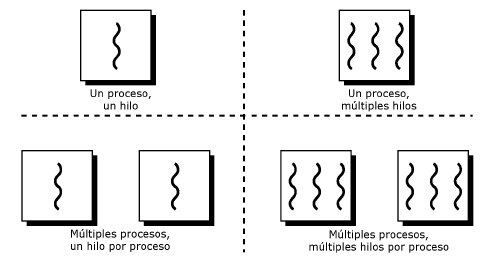
\includegraphics[scale=0.5]{Hilos.png}
      \caption{Hilos y procesos. Tomado de \cite{2}}
      \label{fig:Hilos}
   \end{figure}
\begin{thebibliography}{0}
  \bibitem {1} Qué son los hilos de un procesador.Diferencias con los núcleos.(2019).Profesional Review.
  https://www.profesionalreview.com/2019/04/03/que-son-los-hilos-de-un-procesador/Que-son-los-hilos-de-procesamiento-o-threads
  \bibitem{2} Programación con hilos.(2014). Sebastian Castro. https://prezi.com/zligxav4or3z/programacion-con-hilos/
  \bibitem{3} Procesos e hilos(s.f). Universidad del país Vasco.https://ocw.ehu.eus/pluginfile.php/12388/mod-resource/content/13/html/Recursos/P04/Procesos-y-threads.html
\end{thebibliography}

\end{document}
